\section{Результаты}

\subsection{Выборочные коэффициенты корреляции}

\begin{table}[H]
	\begin{center}
		\begin{tabular}{|c||c|c|c|}
			\hline
			$size = 20$ & $r$ & $r_s$ & $r_q$ \\ 
			\hline 
			$E(z)$ & 0.00559 & 0.00604 & 0.00180 \\ 
			\hline 
			$E(z^2)$ & 0.05722 & 0.05508 & 0.05388 \\ 
			\hline 
			$D(z)$ & 0.05719 & 0.05504 & 0.05388 \\ 
			\hline \hline 
			$size = 60$ & $r$ & $r_s$ & $r_q$ \\ 
			\hline 
			$E(z)$ & -0.00476 & -0.00386 & -0.00260 \\ 
			\hline 
			$E(z^2)$ & 0.01807 & 0.01819 & 0.01728 \\ 
			\hline 
			$D(z)$ & 0.01805 & 0.01817 & 0.01727 \\ 
			\hline \hline 
			$size = 100$ & $r$ & $r_s$ & $r_q$ \\ 
			\hline 
			$E(z)$ & -0.00309 & -0.00270 & -0.00348 \\ 
			\hline 
			$E(z^2)$ & 0.00980 & 0.00990 & 0.01003 \\ 
			\hline 
			$D(z)$ & 0.00979 & 0.00989 & 0.01002 \\ 
			\hline
		\end{tabular}
	\end{center}
	\caption{Двумерное нормальное распределение $\rho = 0$}
\end{table} 

\begin{table}[H]
	\begin{center}
		\begin{tabular}{|c||c|c|c|}
			\hline
			$size = 20$ & $r$ & $r_s$ & $r_q$ \\ 
			\hline 
			$E(z)$ & 0.48728 & 0.46564 & 0.33940 \\ 
			\hline 
			$E(z^2)$ & 0.27003 & 0.25306 & 0.16420 \\ 
			\hline 
			$D(z)$ & 0.03259 & 0.03624 & 0.04901 \\ 
			\hline \hline 
			$size = 60$ & $r$ & $r_s$ & $r_q$ \\ 
			\hline 
			$E(z)$ & 0.49830 & 0.47663 & 0.33273 \\ 
			\hline 
			$E(z^2)$ & 0.25762 & 0.23768 & 0.12535 \\ 
			\hline 
			$D(z)$ & 0.00932 & 0.01050 & 0.01464 \\ 
			\hline \hline 
			$size = 100$ & $r$ & $r_s$ & $r_q$ \\ 
			\hline 
			$E(z)$ & 0.49535 & 0.47482 & 0.32672 \\ 
			\hline 
			$E(z^2)$ & 0.25123 & 0.23225 & 0.11668 \\ 
			\hline 
			$D(z)$ & 0.00586 & 0.00679 & 0.00993 \\ 
			\hline 
		\end{tabular}
	\end{center}
	\caption{Двумерное нормальное распределение $\rho = 0.5$}
\end{table} 

\begin{table}[H]
	\begin{center}
		\begin{tabular}{|c||c|c|c|}
		\hline
		$size = 20$ & $r$ & $r_s$ & $r_q$ \\ 
		\hline 
		$E(z)$ & 0.89710 & 0.86851 & 0.69720 \\ 
		\hline 
		$E(z^2)$ & 0.80705 & 0.75889 & 0.51384 \\ 
		\hline 
		$D(z)$ & 0.00225 & 0.00458 & 0.02775 \\ 
		\hline \hline 
		$size = 60$ & $r$ & $r_s$ & $r_q$ \\ 
		\hline 
		$E(z)$ & 0.89786 & 0.88201 & 0.70300 \\ 
		\hline 
		$E(z^2)$ & 0.80679 & 0.77903 & 0.50279 \\ 
		\hline 
		$D(z)$ & 0.00064 & 0.00110 & 0.00858 \\ 
		\hline \hline 
		$size = 100$ & $r$ & $r_s$ & $r_q$ \\ 
		\hline 
		$E(z)$ & 0.89863 & 0.88605 & 0.70752 \\ 
		\hline 
		$E(z^2)$ & 0.80794 & 0.78571 & 0.50582 \\ 
		\hline 
		$D(z)$ & 0.00039 & 0.00062 & 0.00524 \\ 
		\hline 
		\end{tabular}
	\end{center}
	\caption{Двумерное нормальное распределение $\rho = 0.9$}
\end{table} 

\begin{table}[H]
	\begin{center}
		\begin{tabular}{|c||c|c|c|}
			\hline
			$size = 20$ & $r$ & $r_s$ & $r_q$ \\ 
			\hline 
			$E(z)$ & 0.78243 & 0.74746 & 0.56700 \\ 
			\hline 
			$E(z^2)$ & 0.62071 & 0.57078 & 0.35628 \\ 
			\hline 
			$D(z)$ & 0.00851 & 0.01208 & 0.03479 \\ 
			\hline \hline 
			$size = 60$ & $r$ & $r_s$ & $r_q$ \\ 
			\hline 
			$E(z)$ & 0.79042 & 0.77002 & 0.58047 \\ 
			\hline 
			$E(z^2)$ & 0.62747 & 0.59652 & 0.34752 \\ 
			\hline 
			$D(z)$ & 0.00271 & 0.00359 & 0.01058 \\ 
			\hline \hline 
			$size = 100$ & $r$ & $r_s$ & $r_q$ \\ 
			\hline 
			$E(z)$ & 0.78787 & 0.76874 & 0.57448 \\ 
			\hline 
			$E(z^2)$ & 0.62225 & 0.59306 & 0.33664 \\ 
			\hline 
			$D(z)$ & 0.00151 & 0.00210 & 0.00662 \\ 
			\hline 
		\end{tabular}
	\end{center}
	\caption{Смесь нормальных распределений}
\end{table} 

\subsection{Эллипсы рассеивания}

Для уравнения эллипса выбиралась константа равная $const = 3\sigma$

\begin{figure}[H]
	\begin{tabular}{cccc}
		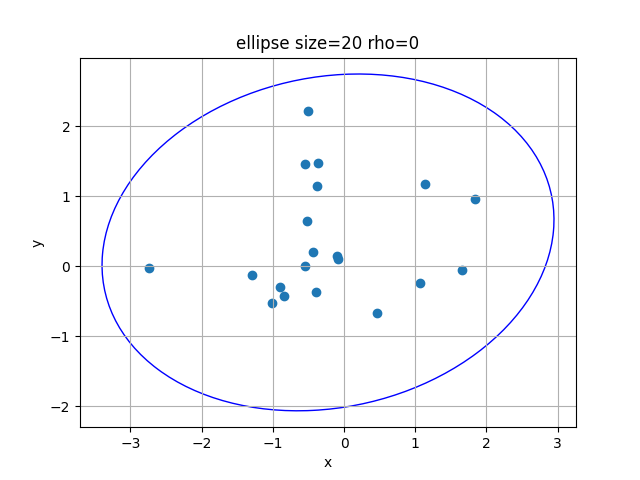
\includegraphics[scale=0.3]{ellipse_20_0.png}
		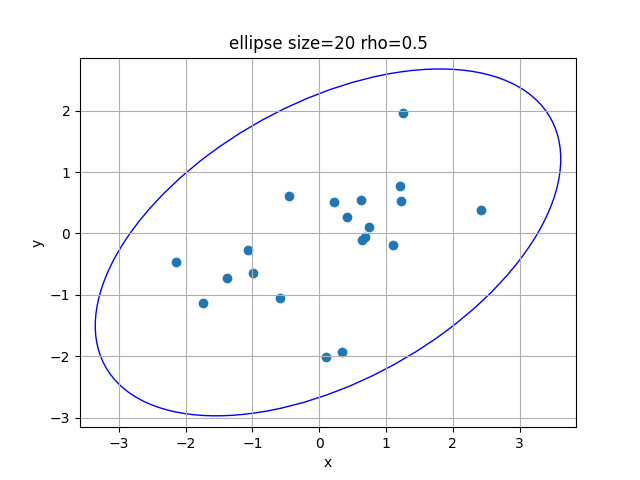
\includegraphics[scale=0.3]{ellipse_20_0.5.png}
		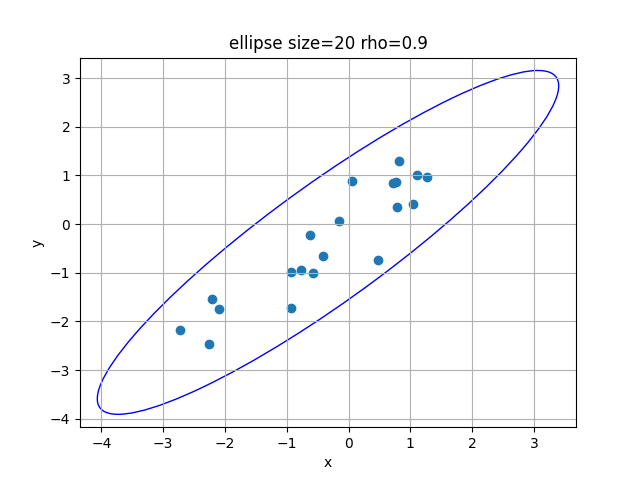
\includegraphics[scale=0.3]{ellipse_20_0.9.png}
		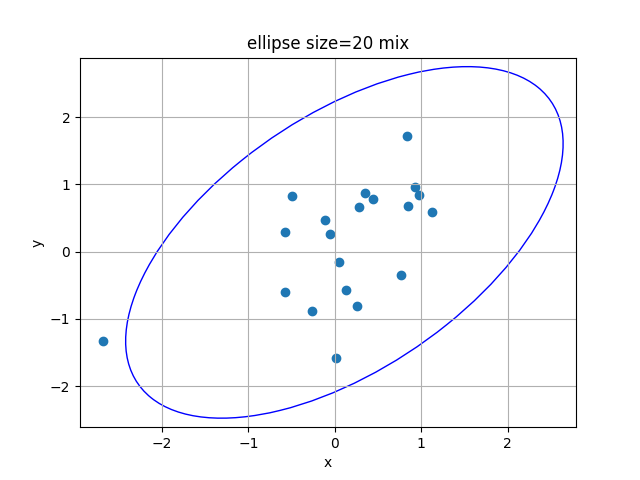
\includegraphics[scale=0.3]{ellipse_20_mix.png}
	\end{tabular}
	\caption{Эллипсы рассеивания для двумерного нормального распределения и смеси нормальных распределений, n = 20}
\end{figure}

\begin{figure}[H]
	\begin{tabular}{cccc}
		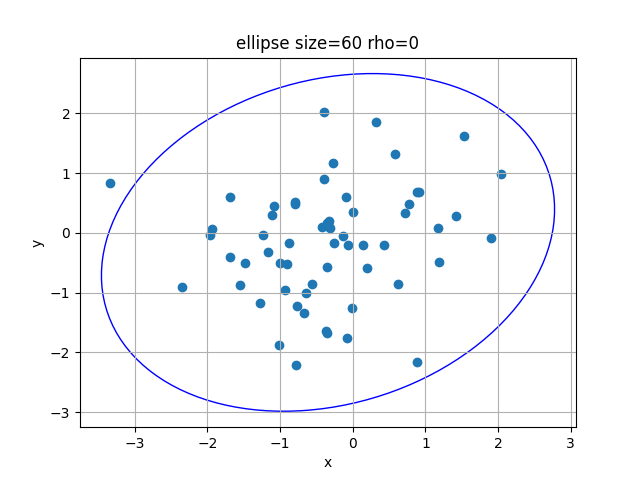
\includegraphics[scale=0.3]{ellipse_60_0.png}
		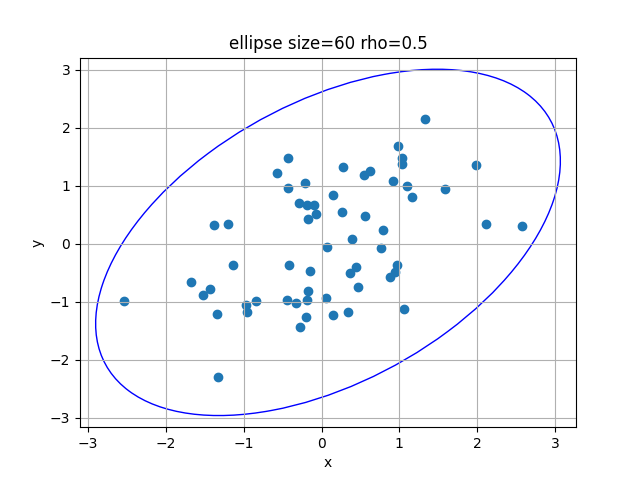
\includegraphics[scale=0.3]{ellipse_60_0.5.png}
		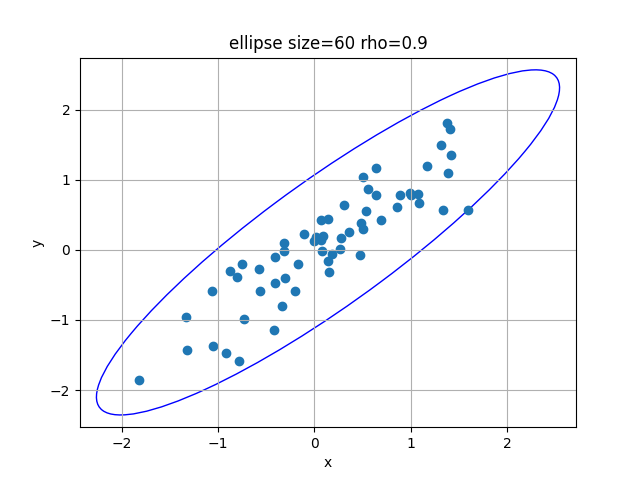
\includegraphics[scale=0.3]{ellipse_60_0.9.png}
		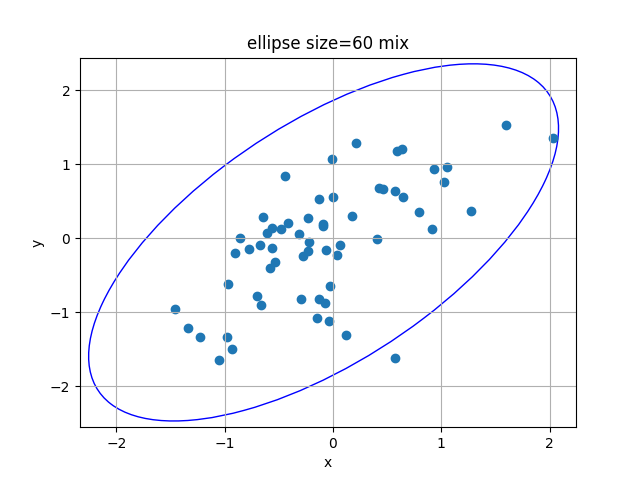
\includegraphics[scale=0.3]{ellipse_60_mix.png}
	\end{tabular}
	\caption{Эллипсы рассеивания для двумерного нормального распределения и смеси нормальных распределений, n = 60}
\end{figure}

\begin{figure}[H]
	\begin{tabular}{cccc}
		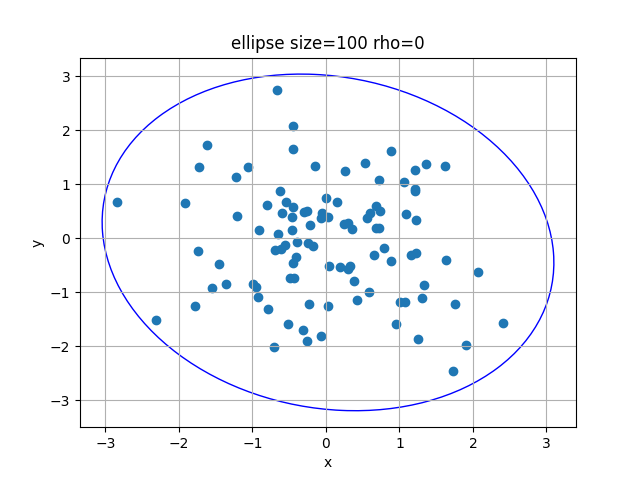
\includegraphics[scale=0.3]{ellipse_100_0.png}
		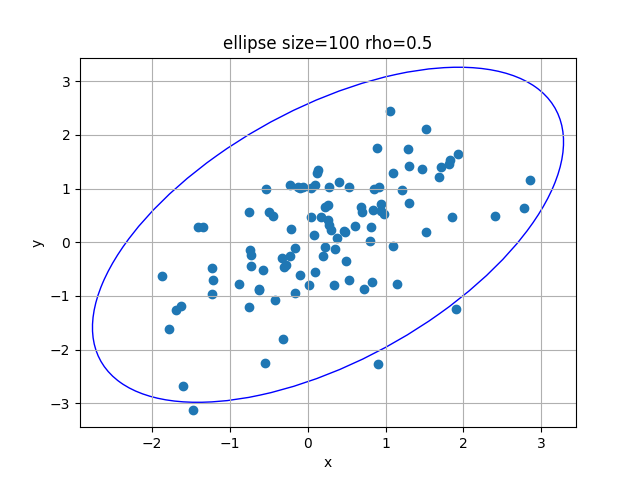
\includegraphics[scale=0.3]{ellipse_100_0.5.png}
		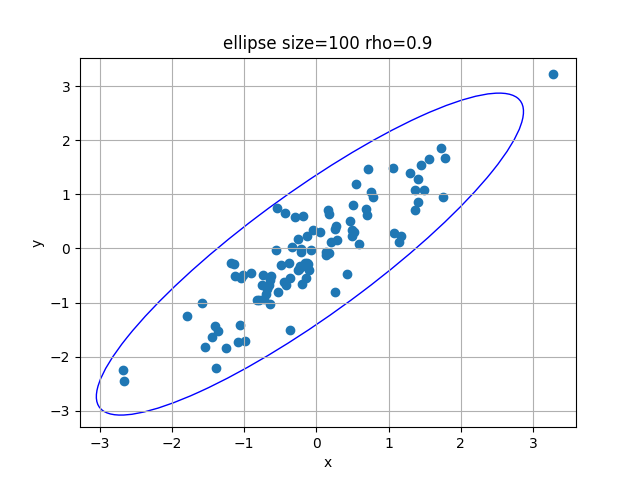
\includegraphics[scale=0.3]{ellipse_100_0.9.png}
		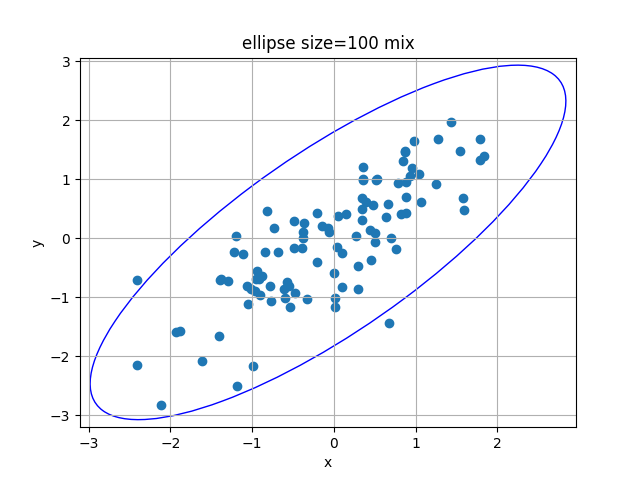
\includegraphics[scale=0.3]{ellipse_100_mix.png}
	\end{tabular}
	\caption{Эллипсы рассеивания для двумерного нормального распределения и смеси нормальных распределений, n = 100}
\end{figure}
